\documentclass[twoside]{book}

% Packages required by doxygen
\usepackage{fixltx2e}
\usepackage{calc}
\usepackage{doxygen}
\usepackage[export]{adjustbox} % also loads graphicx
\usepackage{graphicx}
\usepackage[utf8]{inputenc}
\usepackage{makeidx}
\usepackage{multicol}
\usepackage{multirow}
\PassOptionsToPackage{warn}{textcomp}
\usepackage{textcomp}
\usepackage[nointegrals]{wasysym}
\usepackage[table]{xcolor}

% Font selection
\usepackage[T1]{fontenc}
\usepackage[scaled=.90]{helvet}
\usepackage{courier}
\usepackage{amssymb}
\usepackage{sectsty}
\renewcommand{\familydefault}{\sfdefault}
\allsectionsfont{%
  \fontseries{bc}\selectfont%
  \color{darkgray}%
}
\renewcommand{\DoxyLabelFont}{%
  \fontseries{bc}\selectfont%
  \color{darkgray}%
}
\newcommand{\+}{\discretionary{\mbox{\scriptsize$\hookleftarrow$}}{}{}}

% Page & text layout
\usepackage{geometry}
\geometry{%
  a4paper,%
  top=2.5cm,%
  bottom=2.5cm,%
  left=2.5cm,%
  right=2.5cm%
}
\tolerance=750
\hfuzz=15pt
\hbadness=750
\setlength{\emergencystretch}{15pt}
\setlength{\parindent}{0cm}
\setlength{\parskip}{3ex plus 2ex minus 2ex}
\makeatletter
\renewcommand{\paragraph}{%
  \@startsection{paragraph}{4}{0ex}{-1.0ex}{1.0ex}{%
    \normalfont\normalsize\bfseries\SS@parafont%
  }%
}
\renewcommand{\subparagraph}{%
  \@startsection{subparagraph}{5}{0ex}{-1.0ex}{1.0ex}{%
    \normalfont\normalsize\bfseries\SS@subparafont%
  }%
}
\makeatother

% Headers & footers
\usepackage{fancyhdr}
\pagestyle{fancyplain}
\fancyhead[LE]{\fancyplain{}{\bfseries\thepage}}
\fancyhead[CE]{\fancyplain{}{}}
\fancyhead[RE]{\fancyplain{}{\bfseries\leftmark}}
\fancyhead[LO]{\fancyplain{}{\bfseries\rightmark}}
\fancyhead[CO]{\fancyplain{}{}}
\fancyhead[RO]{\fancyplain{}{\bfseries\thepage}}
\fancyfoot[LE]{\fancyplain{}{}}
\fancyfoot[CE]{\fancyplain{}{}}
\fancyfoot[RE]{\fancyplain{}{\bfseries\scriptsize Generated by Doxygen }}
\fancyfoot[LO]{\fancyplain{}{\bfseries\scriptsize Generated by Doxygen }}
\fancyfoot[CO]{\fancyplain{}{}}
\fancyfoot[RO]{\fancyplain{}{}}
\renewcommand{\footrulewidth}{0.4pt}
\renewcommand{\chaptermark}[1]{%
  \markboth{#1}{}%
}
\renewcommand{\sectionmark}[1]{%
  \markright{\thesection\ #1}%
}

% Indices & bibliography
\usepackage{natbib}
\usepackage[titles]{tocloft}
\setcounter{tocdepth}{3}
\setcounter{secnumdepth}{5}
\makeindex

% Hyperlinks (required, but should be loaded last)
\usepackage{ifpdf}
\ifpdf
  \usepackage[pdftex,pagebackref=true]{hyperref}
\else
  \usepackage[ps2pdf,pagebackref=true]{hyperref}
\fi
\hypersetup{%
  colorlinks=true,%
  linkcolor=blue,%
  citecolor=blue,%
  unicode%
}

% Custom commands
\newcommand{\clearemptydoublepage}{%
  \newpage{\pagestyle{empty}\cleardoublepage}%
}

\usepackage{caption}
\captionsetup{labelsep=space,justification=centering,font={bf},singlelinecheck=off,skip=4pt,position=top}

%===== C O N T E N T S =====

\begin{document}

% Titlepage & ToC
\hypersetup{pageanchor=false,
             bookmarksnumbered=true,
             pdfencoding=unicode
            }
\pagenumbering{roman}
\begin{titlepage}
\vspace*{7cm}
\begin{center}%
{\Large My Project }\\
\vspace*{1cm}
{\large Generated by Doxygen 1.8.11}\\
\end{center}
\end{titlepage}
\clearemptydoublepage
\tableofcontents
\clearemptydoublepage
\pagenumbering{arabic}
\hypersetup{pageanchor=true}

%--- Begin generated contents ---
\chapter{Class Index}
\section{Class List}
Here are the classes, structs, unions and interfaces with brief descriptions\+:\begin{DoxyCompactList}
\item\contentsline{section}{\hyperlink{structnode}{node} }{\pageref{structnode}}{}
\item\contentsline{section}{\hyperlink{structnode1}{node1} }{\pageref{structnode1}}{}
\item\contentsline{section}{\hyperlink{structnode__info}{node\+\_\+info} }{\pageref{structnode__info}}{}
\end{DoxyCompactList}

\chapter{File Index}
\section{File List}
Here is a list of all files with brief descriptions\+:\begin{DoxyCompactList}
\item\contentsline{section}{\hyperlink{Lab1_8c}{Lab1.\+c} }{\pageref{Lab1_8c}}{}
\end{DoxyCompactList}

\chapter{Class Documentation}
\hypertarget{classBall}{}\section{Ball Class Reference}
\label{classBall}\index{Ball@{Ball}}


{\ttfamily \#include $<$Ball.\+h$>$}

\subsection*{Public Member Functions}
\begin{DoxyCompactItemize}
\item 
\hyperlink{classBall_abfa746ecf867895ba38498da7f19ed28}{Ball} (double \hyperlink{classBall_a60894aab5e27e93bacf2393b9110a049}{x}=0.\+0, double \hyperlink{classBall_a17d73231eab81d0e74cf28d0068fe5cb}{y}=0.\+0, double \hyperlink{classBall_aa5e337441f77e5c2b904dbd4340eaa20}{x\+Speed}=0.\+0, double \hyperlink{classBall_ab69d19321c76e52ef393c83d0d476f91}{y\+Speed}=0.\+0)
\item 
double \hyperlink{classBall_a480a1d4547fea337598d6d5b7fb83d8f}{getX} () const 
\item 
void \hyperlink{classBall_a5499dc9c66f5f79c535ca970b02a9cee}{setX} (double \hyperlink{classBall_a60894aab5e27e93bacf2393b9110a049}{x})
\item 
double \hyperlink{classBall_a28a7fe3223d2c192e0eefaa75074e820}{getY} () const 
\item 
void \hyperlink{classBall_a3216c6c42326d379f4a884993bea7e70}{setY} (double \hyperlink{classBall_a17d73231eab81d0e74cf28d0068fe5cb}{y})
\item 
double \hyperlink{classBall_a0cd3a4b0c425106cc6de1a3c570befab}{get\+X\+Speed} () const 
\item 
void \hyperlink{classBall_a7e60c76532fc86f537b46c93f22d989b}{set\+X\+Speed} (double \hyperlink{classBall_aa5e337441f77e5c2b904dbd4340eaa20}{x\+Speed})
\item 
double \hyperlink{classBall_a6286edef4057f1d13e56712eb3975d50}{get\+Y\+Speed} () const 
\item 
void \hyperlink{classBall_ab5fddfb821ae6e06aa3237f4ebd4bb84}{set\+Y\+Speed} (double \hyperlink{classBall_ab69d19321c76e52ef393c83d0d476f91}{y\+Speed})
\item 
void \hyperlink{classBall_af38e5a6a3556b833cff90c2cd5292713}{set\+XY} (double \hyperlink{classBall_a60894aab5e27e93bacf2393b9110a049}{x}, double \hyperlink{classBall_a17d73231eab81d0e74cf28d0068fe5cb}{y})
\item 
void \hyperlink{classBall_a1063b6a3532786b7147fad5e07182a45}{set\+X\+Y\+Speed} (double \hyperlink{classBall_aa5e337441f77e5c2b904dbd4340eaa20}{x\+Speed}, double \hyperlink{classBall_ab69d19321c76e52ef393c83d0d476f91}{y\+Speed})
\item 
void \hyperlink{classBall_a05228e822d67b25baf715cf09c325494}{move} ()
\item 
void \hyperlink{classBall_afb29247bbe8aa061a1212a0bd3d7c4b8}{print} () const 
\end{DoxyCompactItemize}
\subsection*{Private Attributes}
\begin{DoxyCompactItemize}
\item 
double \hyperlink{classBall_a60894aab5e27e93bacf2393b9110a049}{x}
\item 
double \hyperlink{classBall_a17d73231eab81d0e74cf28d0068fe5cb}{y}
\item 
double \hyperlink{classBall_aa5e337441f77e5c2b904dbd4340eaa20}{x\+Speed}
\item 
double \hyperlink{classBall_ab69d19321c76e52ef393c83d0d476f91}{y\+Speed}
\end{DoxyCompactItemize}


\subsection{Constructor \& Destructor Documentation}
\index{Ball@{Ball}!Ball@{Ball}}
\index{Ball@{Ball}!Ball@{Ball}}
\subsubsection[{\texorpdfstring{Ball(double x=0.\+0, double y=0.\+0, double x\+Speed=0.\+0, double y\+Speed=0.\+0)}{Ball(double x=0.0, double y=0.0, double xSpeed=0.0, double ySpeed=0.0)}}]{\setlength{\rightskip}{0pt plus 5cm}Ball\+::\+Ball (
\begin{DoxyParamCaption}
\item[{double}]{x = {\ttfamily 0.0}, }
\item[{double}]{y = {\ttfamily 0.0}, }
\item[{double}]{x\+Speed = {\ttfamily 0.0}, }
\item[{double}]{y\+Speed = {\ttfamily 0.0}}
\end{DoxyParamCaption}
)}\hypertarget{classBall_abfa746ecf867895ba38498da7f19ed28}{}\label{classBall_abfa746ecf867895ba38498da7f19ed28}

\begin{DoxyCode}
9       : \hyperlink{classBall_a60894aab5e27e93bacf2393b9110a049}{x}(\hyperlink{classBall_a60894aab5e27e93bacf2393b9110a049}{x}), \hyperlink{classBall_a17d73231eab81d0e74cf28d0068fe5cb}{y}(\hyperlink{classBall_a17d73231eab81d0e74cf28d0068fe5cb}{y}), \hyperlink{classBall_aa5e337441f77e5c2b904dbd4340eaa20}{xSpeed}(\hyperlink{classBall_aa5e337441f77e5c2b904dbd4340eaa20}{xSpeed}), \hyperlink{classBall_ab69d19321c76e52ef393c83d0d476f91}{ySpeed}(\hyperlink{classBall_ab69d19321c76e52ef393c83d0d476f91}{ySpeed}) \{ \}  \textcolor{comment}{// use member
       initializer list}
\end{DoxyCode}


\subsection{Member Function Documentation}
\index{Ball@{Ball}!getX@{getX}}
\index{getX@{getX}!Ball@{Ball}}
\subsubsection[{\texorpdfstring{get\+X() const }{getX() const }}]{\setlength{\rightskip}{0pt plus 5cm}double Ball\+::getX (
\begin{DoxyParamCaption}
{}
\end{DoxyParamCaption}
) const}\hypertarget{classBall_a480a1d4547fea337598d6d5b7fb83d8f}{}\label{classBall_a480a1d4547fea337598d6d5b7fb83d8f}

\begin{DoxyCode}
12                         \{
13    \textcolor{keywordflow}{return} \hyperlink{classBall_a60894aab5e27e93bacf2393b9110a049}{x};
14 \}
\end{DoxyCode}
\index{Ball@{Ball}!get\+X\+Speed@{get\+X\+Speed}}
\index{get\+X\+Speed@{get\+X\+Speed}!Ball@{Ball}}
\subsubsection[{\texorpdfstring{get\+X\+Speed() const }{getXSpeed() const }}]{\setlength{\rightskip}{0pt plus 5cm}double Ball\+::get\+X\+Speed (
\begin{DoxyParamCaption}
{}
\end{DoxyParamCaption}
) const}\hypertarget{classBall_a0cd3a4b0c425106cc6de1a3c570befab}{}\label{classBall_a0cd3a4b0c425106cc6de1a3c570befab}

\begin{DoxyCode}
24                              \{
25    \textcolor{keywordflow}{return} \hyperlink{classBall_aa5e337441f77e5c2b904dbd4340eaa20}{xSpeed};
26 \}
\end{DoxyCode}
\index{Ball@{Ball}!getY@{getY}}
\index{getY@{getY}!Ball@{Ball}}
\subsubsection[{\texorpdfstring{get\+Y() const }{getY() const }}]{\setlength{\rightskip}{0pt plus 5cm}double Ball\+::getY (
\begin{DoxyParamCaption}
{}
\end{DoxyParamCaption}
) const}\hypertarget{classBall_a28a7fe3223d2c192e0eefaa75074e820}{}\label{classBall_a28a7fe3223d2c192e0eefaa75074e820}

\begin{DoxyCode}
15                         \{
16    \textcolor{keywordflow}{return} \hyperlink{classBall_a17d73231eab81d0e74cf28d0068fe5cb}{y};
17 \}
\end{DoxyCode}
\index{Ball@{Ball}!get\+Y\+Speed@{get\+Y\+Speed}}
\index{get\+Y\+Speed@{get\+Y\+Speed}!Ball@{Ball}}
\subsubsection[{\texorpdfstring{get\+Y\+Speed() const }{getYSpeed() const }}]{\setlength{\rightskip}{0pt plus 5cm}double Ball\+::get\+Y\+Speed (
\begin{DoxyParamCaption}
{}
\end{DoxyParamCaption}
) const}\hypertarget{classBall_a6286edef4057f1d13e56712eb3975d50}{}\label{classBall_a6286edef4057f1d13e56712eb3975d50}

\begin{DoxyCode}
27                              \{
28    \textcolor{keywordflow}{return} \hyperlink{classBall_ab69d19321c76e52ef393c83d0d476f91}{ySpeed};
29 \}
\end{DoxyCode}
\index{Ball@{Ball}!move@{move}}
\index{move@{move}!Ball@{Ball}}
\subsubsection[{\texorpdfstring{move()}{move()}}]{\setlength{\rightskip}{0pt plus 5cm}void Ball\+::move (
\begin{DoxyParamCaption}
{}
\end{DoxyParamCaption}
)}\hypertarget{classBall_a05228e822d67b25baf715cf09c325494}{}\label{classBall_a05228e822d67b25baf715cf09c325494}

\begin{DoxyCode}
50                 \{
51    \hyperlink{classBall_a5499dc9c66f5f79c535ca970b02a9cee}{setX}(\hyperlink{classBall_a60894aab5e27e93bacf2393b9110a049}{x} + \hyperlink{classBall_aa5e337441f77e5c2b904dbd4340eaa20}{xSpeed}); \textcolor{comment}{// increment x by xSpeed}
52    \hyperlink{classBall_a3216c6c42326d379f4a884993bea7e70}{setY}(\hyperlink{classBall_a17d73231eab81d0e74cf28d0068fe5cb}{y} + \hyperlink{classBall_ab69d19321c76e52ef393c83d0d476f91}{ySpeed}); \textcolor{comment}{// increment y by ySpeed}
53 \}
\end{DoxyCode}


Here is the call graph for this function\+:
\nopagebreak
\begin{figure}[H]
\begin{center}
\leavevmode
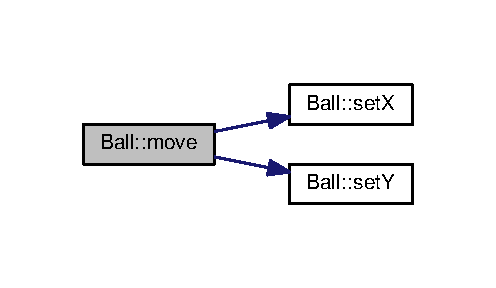
\includegraphics[width=238pt]{classBall_a05228e822d67b25baf715cf09c325494_cgraph}
\end{center}
\end{figure}


\index{Ball@{Ball}!print@{print}}
\index{print@{print}!Ball@{Ball}}
\subsubsection[{\texorpdfstring{print() const }{print() const }}]{\setlength{\rightskip}{0pt plus 5cm}void Ball\+::print (
\begin{DoxyParamCaption}
{}
\end{DoxyParamCaption}
) const}\hypertarget{classBall_afb29247bbe8aa061a1212a0bd3d7c4b8}{}\label{classBall_afb29247bbe8aa061a1212a0bd3d7c4b8}

\begin{DoxyCode}
56                        \{
57    cout << fixed << setprecision(2);
58    cout << \textcolor{stringliteral}{"Ball @ ("} << \hyperlink{classBall_a60894aab5e27e93bacf2393b9110a049}{x} << \textcolor{charliteral}{','} << \hyperlink{classBall_a17d73231eab81d0e74cf28d0068fe5cb}{y} << \textcolor{stringliteral}{") with speed ("}
59         << \hyperlink{classBall_aa5e337441f77e5c2b904dbd4340eaa20}{xSpeed} << \textcolor{charliteral}{','} << \hyperlink{classBall_ab69d19321c76e52ef393c83d0d476f91}{ySpeed} << \textcolor{charliteral}{')'} << endl;
60 \}\end{DoxyCode}
\index{Ball@{Ball}!setX@{setX}}
\index{setX@{setX}!Ball@{Ball}}
\subsubsection[{\texorpdfstring{set\+X(double x)}{setX(double x)}}]{\setlength{\rightskip}{0pt plus 5cm}void Ball\+::setX (
\begin{DoxyParamCaption}
\item[{double}]{x}
\end{DoxyParamCaption}
)}\hypertarget{classBall_a5499dc9c66f5f79c535ca970b02a9cee}{}\label{classBall_a5499dc9c66f5f79c535ca970b02a9cee}

\begin{DoxyCode}
18                         \{
19    this->\hyperlink{classBall_a60894aab5e27e93bacf2393b9110a049}{x} = \hyperlink{classBall_a60894aab5e27e93bacf2393b9110a049}{x};
20 \}
\end{DoxyCode}
\index{Ball@{Ball}!set\+X\+Speed@{set\+X\+Speed}}
\index{set\+X\+Speed@{set\+X\+Speed}!Ball@{Ball}}
\subsubsection[{\texorpdfstring{set\+X\+Speed(double x\+Speed)}{setXSpeed(double xSpeed)}}]{\setlength{\rightskip}{0pt plus 5cm}void Ball\+::set\+X\+Speed (
\begin{DoxyParamCaption}
\item[{double}]{x\+Speed}
\end{DoxyParamCaption}
)}\hypertarget{classBall_a7e60c76532fc86f537b46c93f22d989b}{}\label{classBall_a7e60c76532fc86f537b46c93f22d989b}

\begin{DoxyCode}
30                                   \{
31    this->\hyperlink{classBall_aa5e337441f77e5c2b904dbd4340eaa20}{xSpeed} = \hyperlink{classBall_aa5e337441f77e5c2b904dbd4340eaa20}{xSpeed};
32 \}
\end{DoxyCode}
\index{Ball@{Ball}!set\+XY@{set\+XY}}
\index{set\+XY@{set\+XY}!Ball@{Ball}}
\subsubsection[{\texorpdfstring{set\+X\+Y(double x, double y)}{setXY(double x, double y)}}]{\setlength{\rightskip}{0pt plus 5cm}void Ball\+::set\+XY (
\begin{DoxyParamCaption}
\item[{double}]{x, }
\item[{double}]{y}
\end{DoxyParamCaption}
)}\hypertarget{classBall_af38e5a6a3556b833cff90c2cd5292713}{}\label{classBall_af38e5a6a3556b833cff90c2cd5292713}

\begin{DoxyCode}
38                                    \{
39    \hyperlink{classBall_a5499dc9c66f5f79c535ca970b02a9cee}{setX}(\hyperlink{classBall_a60894aab5e27e93bacf2393b9110a049}{x});
40    \hyperlink{classBall_a3216c6c42326d379f4a884993bea7e70}{setY}(\hyperlink{classBall_a17d73231eab81d0e74cf28d0068fe5cb}{y});
41 \}
\end{DoxyCode}


Here is the call graph for this function\+:
\nopagebreak
\begin{figure}[H]
\begin{center}
\leavevmode
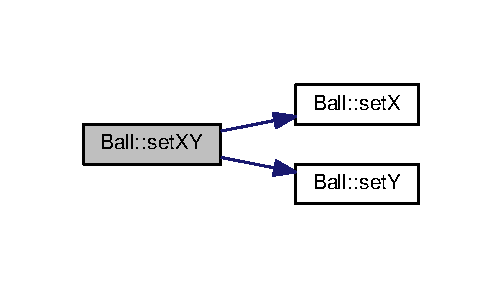
\includegraphics[width=241pt]{classBall_af38e5a6a3556b833cff90c2cd5292713_cgraph}
\end{center}
\end{figure}


\index{Ball@{Ball}!set\+X\+Y\+Speed@{set\+X\+Y\+Speed}}
\index{set\+X\+Y\+Speed@{set\+X\+Y\+Speed}!Ball@{Ball}}
\subsubsection[{\texorpdfstring{set\+X\+Y\+Speed(double x\+Speed, double y\+Speed)}{setXYSpeed(double xSpeed, double ySpeed)}}]{\setlength{\rightskip}{0pt plus 5cm}void Ball\+::set\+X\+Y\+Speed (
\begin{DoxyParamCaption}
\item[{double}]{x\+Speed, }
\item[{double}]{y\+Speed}
\end{DoxyParamCaption}
)}\hypertarget{classBall_a1063b6a3532786b7147fad5e07182a45}{}\label{classBall_a1063b6a3532786b7147fad5e07182a45}

\begin{DoxyCode}
44                                                   \{
45    \hyperlink{classBall_a7e60c76532fc86f537b46c93f22d989b}{setXSpeed}(\hyperlink{classBall_aa5e337441f77e5c2b904dbd4340eaa20}{xSpeed});
46    \hyperlink{classBall_ab5fddfb821ae6e06aa3237f4ebd4bb84}{setYSpeed}(\hyperlink{classBall_ab69d19321c76e52ef393c83d0d476f91}{ySpeed});
47 \}
\end{DoxyCode}


Here is the call graph for this function\+:
\nopagebreak
\begin{figure}[H]
\begin{center}
\leavevmode
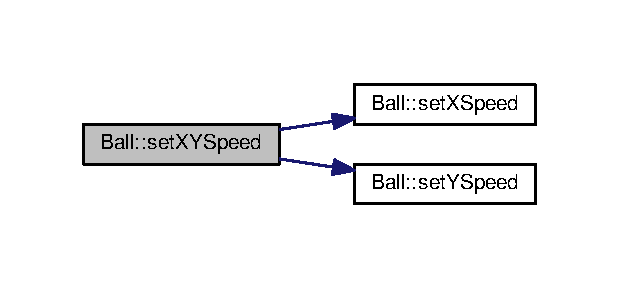
\includegraphics[width=297pt]{classBall_a1063b6a3532786b7147fad5e07182a45_cgraph}
\end{center}
\end{figure}


\index{Ball@{Ball}!setY@{setY}}
\index{setY@{setY}!Ball@{Ball}}
\subsubsection[{\texorpdfstring{set\+Y(double y)}{setY(double y)}}]{\setlength{\rightskip}{0pt plus 5cm}void Ball\+::setY (
\begin{DoxyParamCaption}
\item[{double}]{y}
\end{DoxyParamCaption}
)}\hypertarget{classBall_a3216c6c42326d379f4a884993bea7e70}{}\label{classBall_a3216c6c42326d379f4a884993bea7e70}

\begin{DoxyCode}
21                         \{
22    this->\hyperlink{classBall_a17d73231eab81d0e74cf28d0068fe5cb}{y} = \hyperlink{classBall_a17d73231eab81d0e74cf28d0068fe5cb}{y};
23 \}
\end{DoxyCode}
\index{Ball@{Ball}!set\+Y\+Speed@{set\+Y\+Speed}}
\index{set\+Y\+Speed@{set\+Y\+Speed}!Ball@{Ball}}
\subsubsection[{\texorpdfstring{set\+Y\+Speed(double y\+Speed)}{setYSpeed(double ySpeed)}}]{\setlength{\rightskip}{0pt plus 5cm}void Ball\+::set\+Y\+Speed (
\begin{DoxyParamCaption}
\item[{double}]{y\+Speed}
\end{DoxyParamCaption}
)}\hypertarget{classBall_ab5fddfb821ae6e06aa3237f4ebd4bb84}{}\label{classBall_ab5fddfb821ae6e06aa3237f4ebd4bb84}

\begin{DoxyCode}
33                                   \{
34    this->\hyperlink{classBall_ab69d19321c76e52ef393c83d0d476f91}{ySpeed} = \hyperlink{classBall_ab69d19321c76e52ef393c83d0d476f91}{ySpeed};
35 \}
\end{DoxyCode}


\subsection{Member Data Documentation}
\index{Ball@{Ball}!x@{x}}
\index{x@{x}!Ball@{Ball}}
\subsubsection[{\texorpdfstring{x}{x}}]{\setlength{\rightskip}{0pt plus 5cm}double Ball\+::x\hspace{0.3cm}{\ttfamily [private]}}\hypertarget{classBall_a60894aab5e27e93bacf2393b9110a049}{}\label{classBall_a60894aab5e27e93bacf2393b9110a049}
\index{Ball@{Ball}!x\+Speed@{x\+Speed}}
\index{x\+Speed@{x\+Speed}!Ball@{Ball}}
\subsubsection[{\texorpdfstring{x\+Speed}{xSpeed}}]{\setlength{\rightskip}{0pt plus 5cm}double Ball\+::x\+Speed\hspace{0.3cm}{\ttfamily [private]}}\hypertarget{classBall_aa5e337441f77e5c2b904dbd4340eaa20}{}\label{classBall_aa5e337441f77e5c2b904dbd4340eaa20}
\index{Ball@{Ball}!y@{y}}
\index{y@{y}!Ball@{Ball}}
\subsubsection[{\texorpdfstring{y}{y}}]{\setlength{\rightskip}{0pt plus 5cm}double Ball\+::y\hspace{0.3cm}{\ttfamily [private]}}\hypertarget{classBall_a17d73231eab81d0e74cf28d0068fe5cb}{}\label{classBall_a17d73231eab81d0e74cf28d0068fe5cb}
\index{Ball@{Ball}!y\+Speed@{y\+Speed}}
\index{y\+Speed@{y\+Speed}!Ball@{Ball}}
\subsubsection[{\texorpdfstring{y\+Speed}{ySpeed}}]{\setlength{\rightskip}{0pt plus 5cm}double Ball\+::y\+Speed\hspace{0.3cm}{\ttfamily [private]}}\hypertarget{classBall_ab69d19321c76e52ef393c83d0d476f91}{}\label{classBall_ab69d19321c76e52ef393c83d0d476f91}


The documentation for this class was generated from the following files\+:\begin{DoxyCompactItemize}
\item 
\hyperlink{Ball_8h}{Ball.\+h}\item 
\hyperlink{Ball_8cpp}{Ball.\+cpp}\end{DoxyCompactItemize}

\chapter{File Documentation}
\hypertarget{Ball_8cpp}{}\section{Ball.\+cpp File Reference}
\label{Ball_8cpp}\index{Ball.\+cpp@{Ball.\+cpp}}
{\ttfamily \#include $<$iostream$>$}\\*
{\ttfamily \#include $<$iomanip$>$}\\*
{\ttfamily \#include \char`\"{}Ball.\+h\char`\"{}}\\*
Include dependency graph for Ball.\+cpp\+:
\nopagebreak
\begin{figure}[H]
\begin{center}
\leavevmode
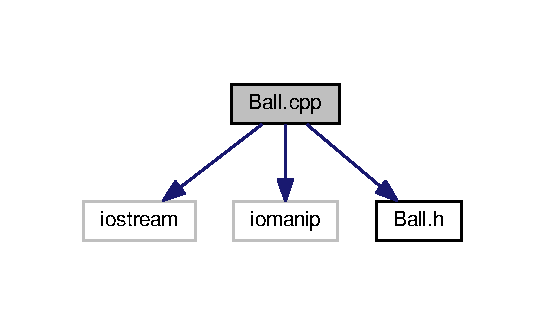
\includegraphics[width=262pt]{Ball_8cpp__incl}
\end{center}
\end{figure}

\hypertarget{Ball_8h}{}\section{Ball.\+h File Reference}
\label{Ball_8h}\index{Ball.\+h@{Ball.\+h}}
This graph shows which files directly or indirectly include this file\+:
\nopagebreak
\begin{figure}[H]
\begin{center}
\leavevmode
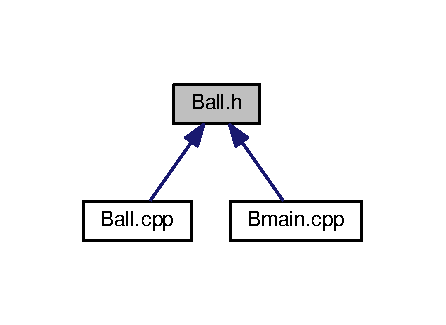
\includegraphics[width=214pt]{Ball_8h__dep__incl}
\end{center}
\end{figure}
\subsection*{Classes}
\begin{DoxyCompactItemize}
\item 
class \hyperlink{classBall}{Ball}
\end{DoxyCompactItemize}

\hypertarget{Bmain_8cpp}{}\section{Bmain.\+cpp File Reference}
\label{Bmain_8cpp}\index{Bmain.\+cpp@{Bmain.\+cpp}}
{\ttfamily \#include $<$iostream$>$}\\*
{\ttfamily \#include \char`\"{}Ball.\+h\char`\"{}}\\*
Include dependency graph for Bmain.\+cpp\+:
\nopagebreak
\begin{figure}[H]
\begin{center}
\leavevmode
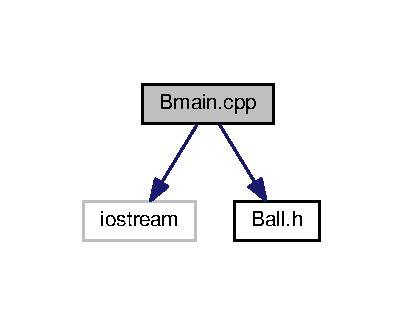
\includegraphics[width=194pt]{Bmain_8cpp__incl}
\end{center}
\end{figure}
\subsection*{Functions}
\begin{DoxyCompactItemize}
\item 
int \hyperlink{Bmain_8cpp_ae66f6b31b5ad750f1fe042a706a4e3d4}{main} ()
\end{DoxyCompactItemize}


\subsection{Function Documentation}
\index{Bmain.\+cpp@{Bmain.\+cpp}!main@{main}}
\index{main@{main}!Bmain.\+cpp@{Bmain.\+cpp}}
\subsubsection[{\texorpdfstring{main()}{main()}}]{\setlength{\rightskip}{0pt plus 5cm}int main (
\begin{DoxyParamCaption}
{}
\end{DoxyParamCaption}
)}\hypertarget{Bmain_8cpp_ae66f6b31b5ad750f1fe042a706a4e3d4}{}\label{Bmain_8cpp_ae66f6b31b5ad750f1fe042a706a4e3d4}

\begin{DoxyCode}
6            \{
7    \hyperlink{classBall}{Ball} ball;
8    ball.\hyperlink{classBall_afb29247bbe8aa061a1212a0bd3d7c4b8}{print}();    \textcolor{comment}{// Ball @ (0.00,0.00) with speed (0.00,0.00)}
9    ball.\hyperlink{classBall_af38e5a6a3556b833cff90c2cd5292713}{setXY}(1.1, 2.2);
10    ball.\hyperlink{classBall_a1063b6a3532786b7147fad5e07182a45}{setXYSpeed}(3.3, 4.4);
11    ball.\hyperlink{classBall_afb29247bbe8aa061a1212a0bd3d7c4b8}{print}();    \textcolor{comment}{// Ball @ (1.10,2.20) with speed (3.30,4.40)}
12    ball.\hyperlink{classBall_a5499dc9c66f5f79c535ca970b02a9cee}{setX}(5.5);
13    ball.\hyperlink{classBall_a3216c6c42326d379f4a884993bea7e70}{setY}(6.6);
14    cout << \textcolor{stringliteral}{"x is "} << ball.\hyperlink{classBall_a480a1d4547fea337598d6d5b7fb83d8f}{getX}() << endl;  \textcolor{comment}{// x is 5.50}
15    cout << \textcolor{stringliteral}{"y is "} << ball.\hyperlink{classBall_a28a7fe3223d2c192e0eefaa75074e820}{getY}() << endl;  \textcolor{comment}{// y is 6.60}
16    ball.\hyperlink{classBall_a05228e822d67b25baf715cf09c325494}{move}();
17    ball.\hyperlink{classBall_afb29247bbe8aa061a1212a0bd3d7c4b8}{print}();    \textcolor{comment}{// Ball @ (8.80,11.00) with speed (3.30,4.40)}
18 \}\end{DoxyCode}


Here is the call graph for this function\+:
\nopagebreak
\begin{figure}[H]
\begin{center}
\leavevmode
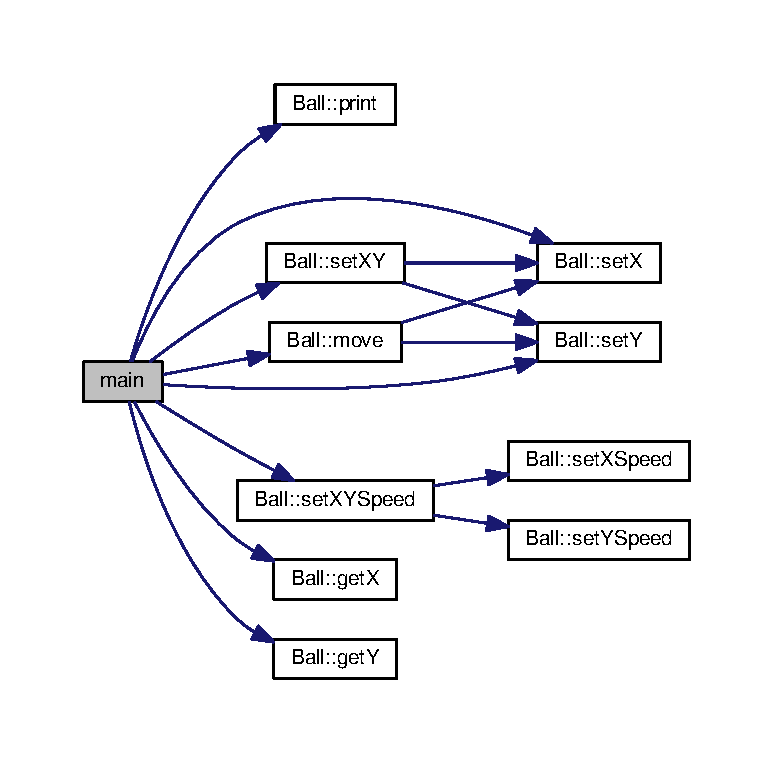
\includegraphics[width=350pt]{Bmain_8cpp_ae66f6b31b5ad750f1fe042a706a4e3d4_cgraph}
\end{center}
\end{figure}



%--- End generated contents ---

% Index
\backmatter
\newpage
\phantomsection
\clearemptydoublepage
\addcontentsline{toc}{chapter}{Index}
\printindex

\end{document}
